\chapter{Attachments}

\section{Learner Rendering Pipeline}
\label{a:studentRenderingPipeline}
\begin{figure}[H]
	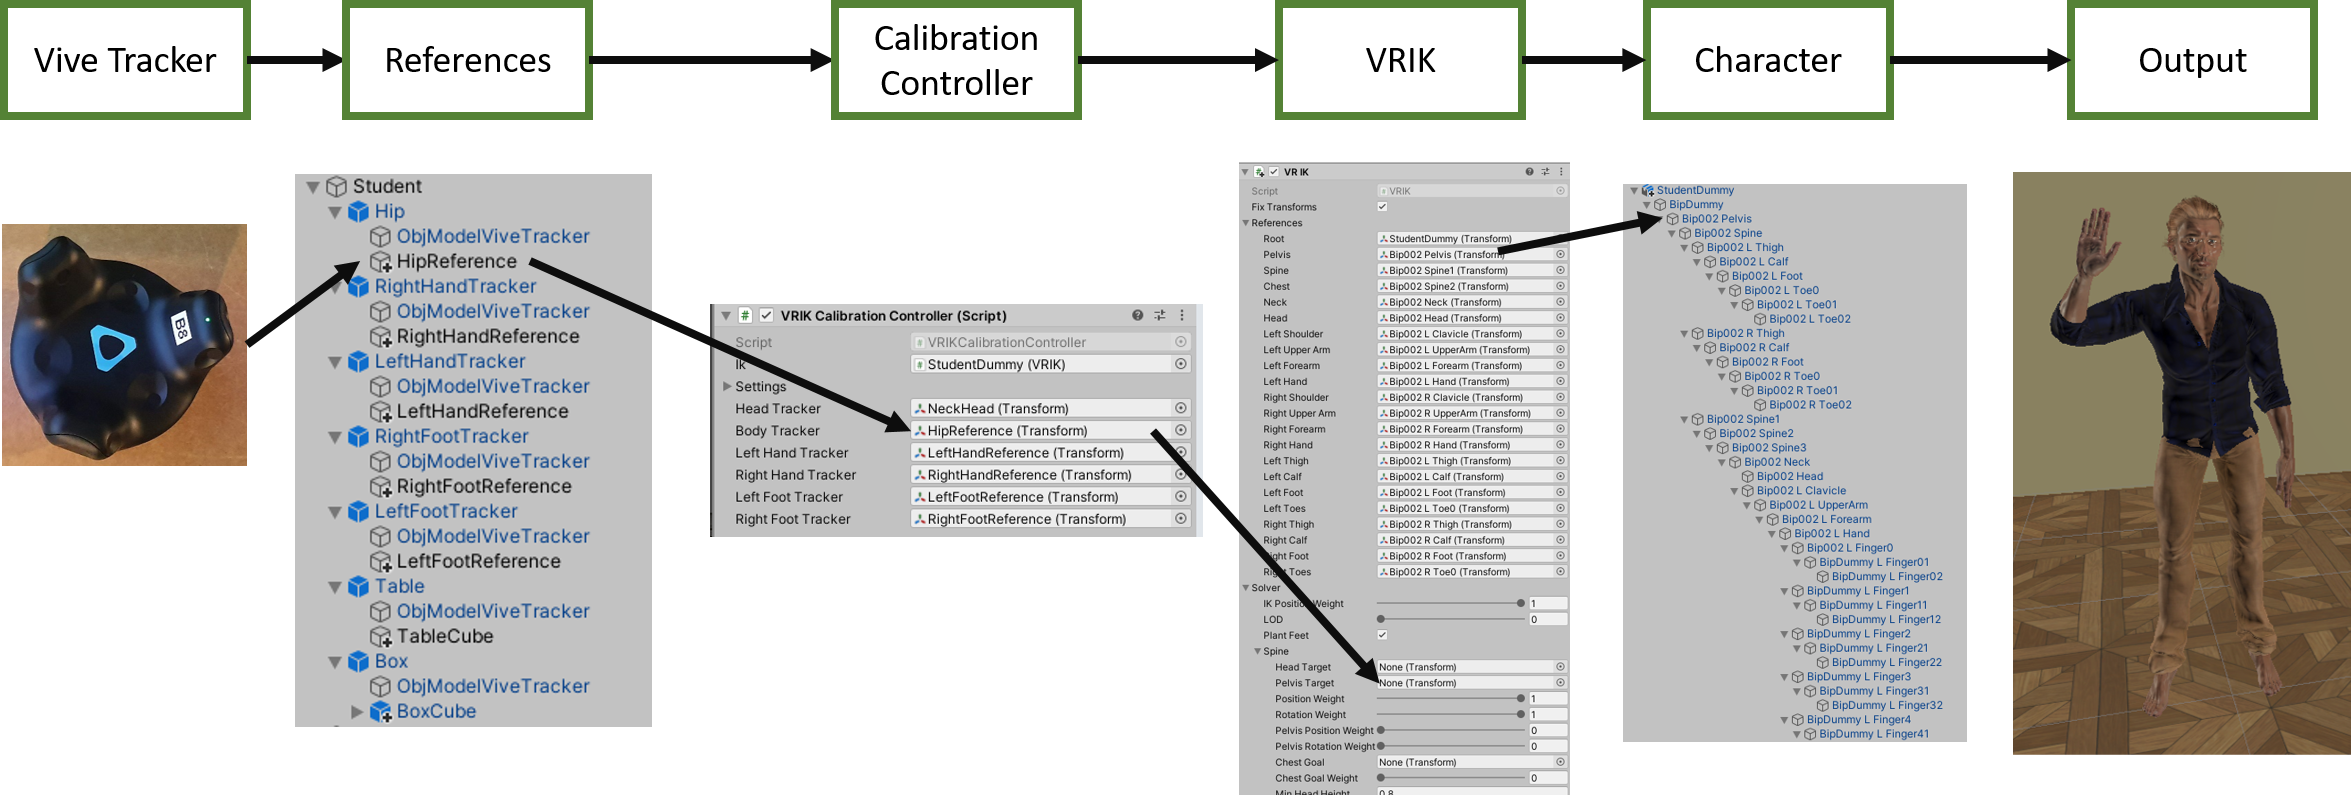
\includegraphics[angle=90,height=18cm]{figures/studentRenderingPipeline.png}
\end{figure}

\newpage
\section{Study Documents}
%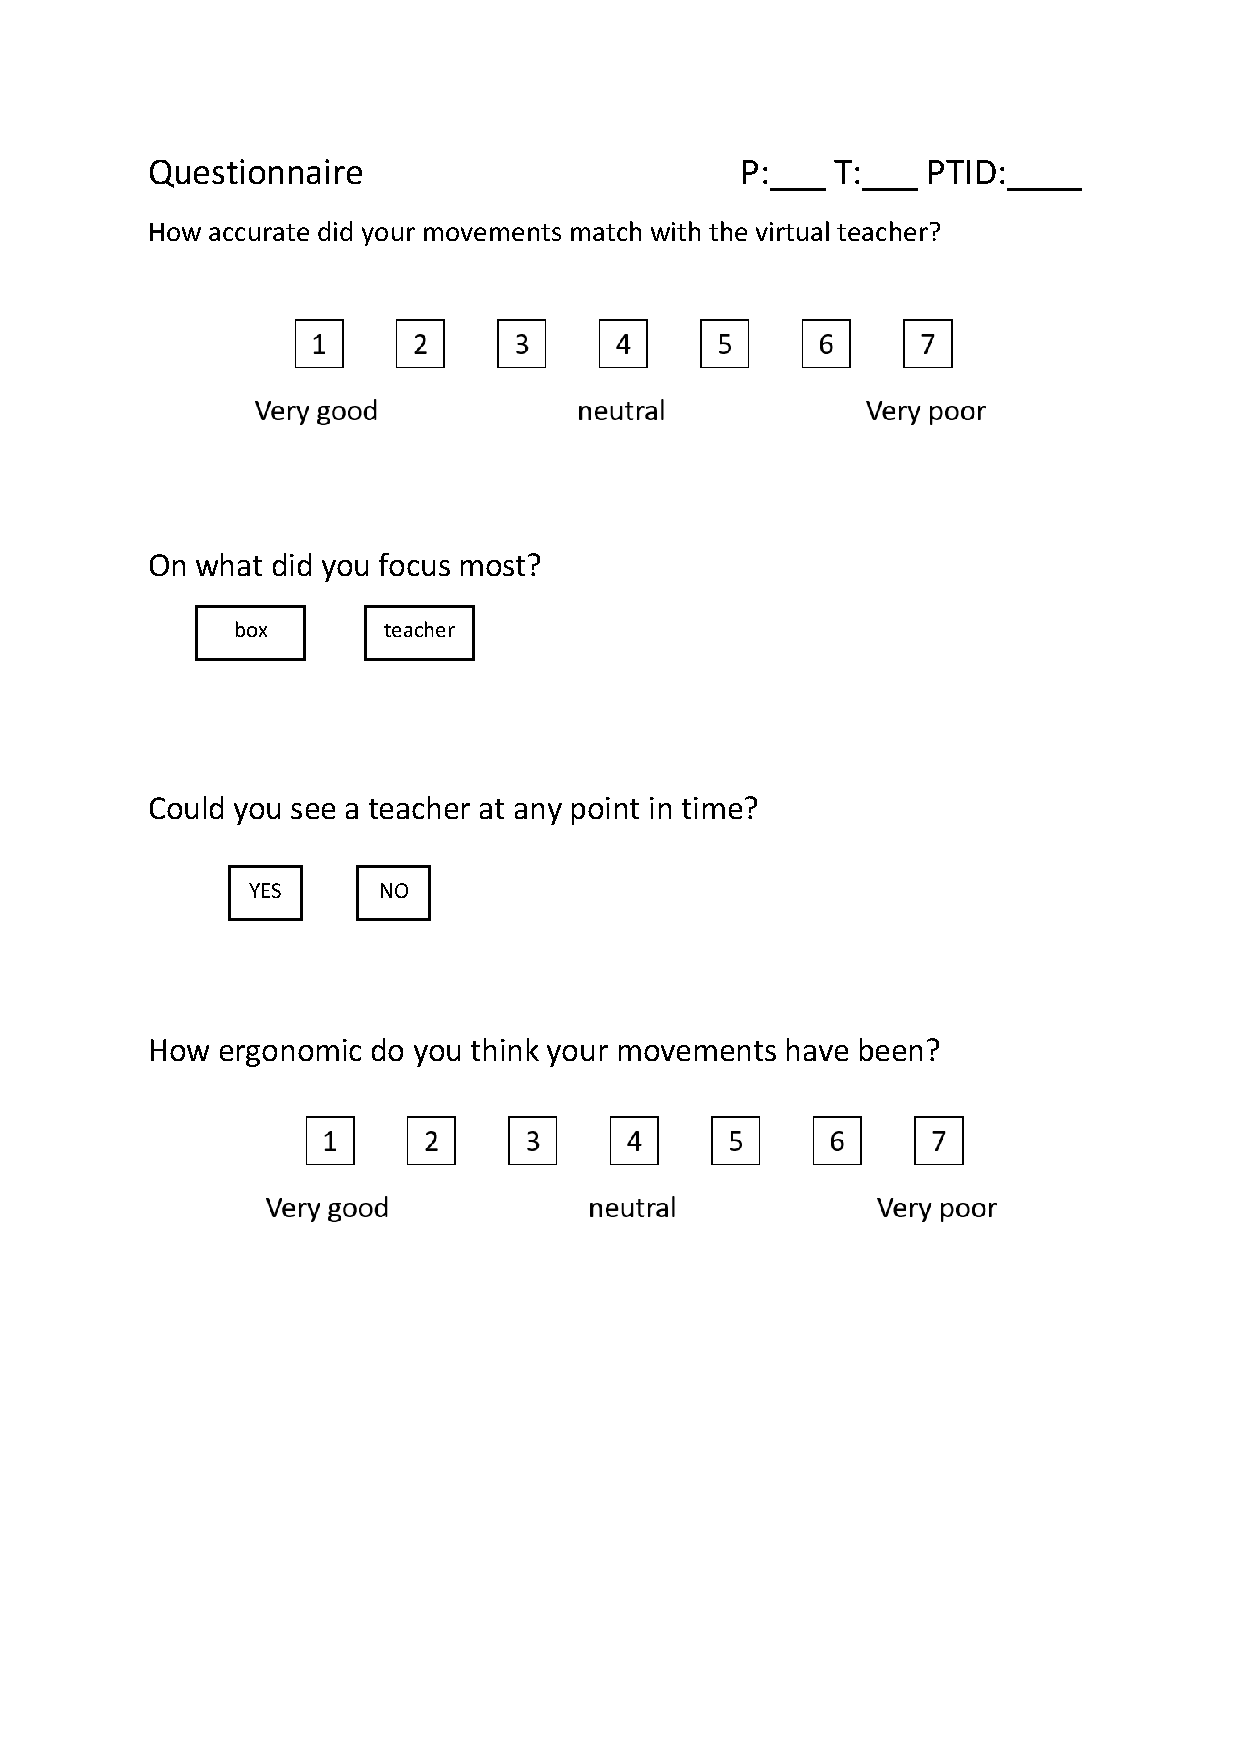
\includepdf[pages=-]{attachments/after_session_questionaire.pdf}
\begin{table}[]
	\begin{tabularx}{\textwidth}{@{}X|XXXXXX@{}}
		\toprule
		& Tai Chi Trainer \cite{thaichichua}   & YouMove \cite{YouMove} & VR Dance Trainer \cite{vrdancetrainer} & OneBody \cite{onebody} & LightGuide \cite{lightguide} & Physio@ Home \cite{physioathome} \\ \midrule
		Perspective &
		Exo-centric,\newline Ego \& augmented exo-centric &
		Exo-centric &
		Exo-centric &
		Ego-centric,\newline exo-centric &
		Ego-centric,\newline exo-centric &
		Exo-centric \\ 
		Task & Tai Chi & Dance (Ballet), abstract & Dance (HipHop)   & Martial Arts         & Abstract   & Shoulder rehab \\ 
		GV   & Avatar, \newline wireframe & Stick figure,\newline avatar     & Avatar           & Stick figure,\newline avatar & Indicators & Indicators     \\ 
		Variable &
		Perspectives,\newline performance &
		VR/video,\newline performance &
		VR/video,\newline performance &
		Training method,\newline performance &
		Visualisations,\newline perspectives,\newline performance &
		Visualisations,\newline performance \\ 
		Results &
		No \newline difference in performance &
		VR better than video &
		VR better than video &
		Ego better than exo &
		Ego better then exo &
		Multi view better than single view \\ 
		\bottomrule
	\end{tabularx}
	\caption[Detailed analysis of related work in seminar thesis.]{Detailed seminar thesis evaluation.}
	\label{tab:rw_overview_detail}
\end{table}